%%%%%%%%%%%%%%%%%%%%%%%%%%%%%%%%%%%%%%%%%%%%%%%%%%%%%%%%%%%%%%%%%%%%%%%%%%%%%%%%

\section{Lecture 5: Snowball Earth}

\textbf{We don't know if it actually happened.}

Scientists agree there was a major change in Earth's climate. Disputes concern
how major.

\subsection{Carbon isotope fractionation}

Bacteria take the lighter isotope $^{12}$C out of water and preferentially
leave out $^{13}$C.

"Default" value for $\delta^{13}$C is -6 (when no factors affect it).
Values of $\delta^{13}$C equal or below -6 mean there is no life at all.

When organic material intakes $^{12}$C, the $\delta^{13}$C in the surrounding
water increases.

\subsection{Port Askaig Tillite Formation, Islay}

\textit{...the material of which the mass is composed have in time, deeper than
we have hitherto suspected, been transported by the agency of ice.} - James
Thomson, F.G.S. 1871 on the stratified rocks of Islay

\subsection{Sturtian (718-658 Myr) and Marinoan (650-635 Myr)}

Similar glaciar rocks as found by Thomson were found everywhere, not only
on Islay. This is surprising because what would glaciar rocks do e.g. in
Australia?

\textbf{Howchin (1908): Sturtian Formation in Sturt river,
Austrailia}

\textbf{isräfflor} - scratches on rocks done by glaciers.

\textbf{Mawson (1949): Elatina Formation, Australia}

\textit{Records of severe glaciation in the late Precambrian are fast
accumulating. So far as can at present be judged, frequent and widespread
refrigerations were a feature of at least middle to late Proterozoic time.
Glaciation is evidenced to the Equators itself.
}
%%%%%%%%%%%%%%%%%%%%%%%%%%%%%%%%%%%%%%%%%%%%%%%%%%%%%%%%%%%%%%%%%%%%%%%%%%%%%%%%
\subsection{Paleomagnetic studies of Gondwana during the Neoproterozoic Era}
Neoproterozoic\footnote{1 billion to 538.8 million years ago}

\begin{figure}[H]
    \centering
    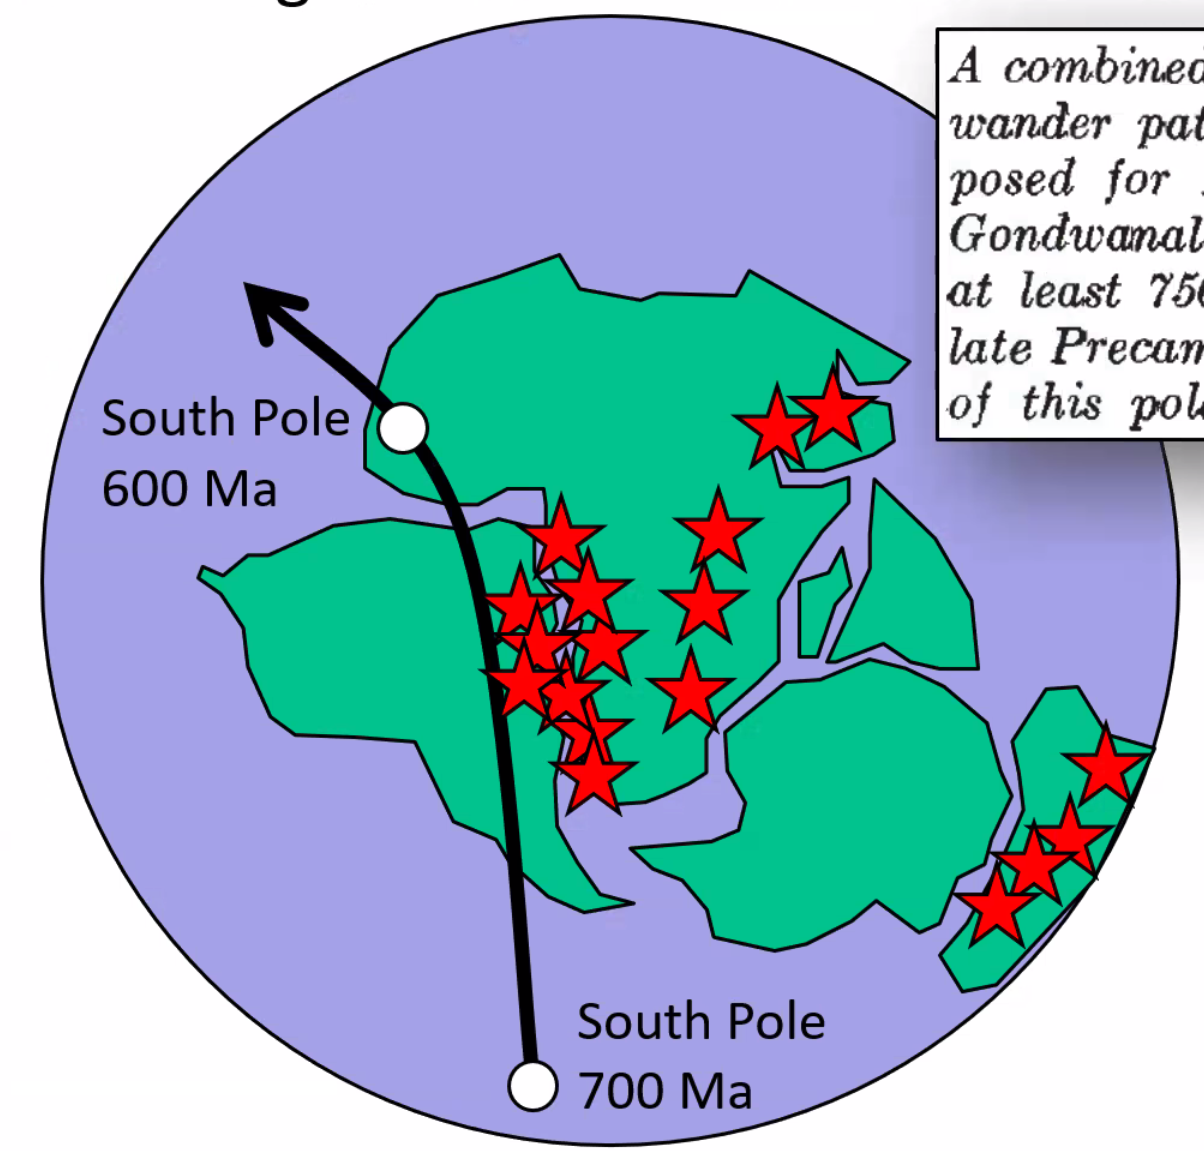
\includegraphics[width=0.75\linewidth]{content/img/gondwana.png}
\end{figure}

\begin{figure}[H]
    \centering
    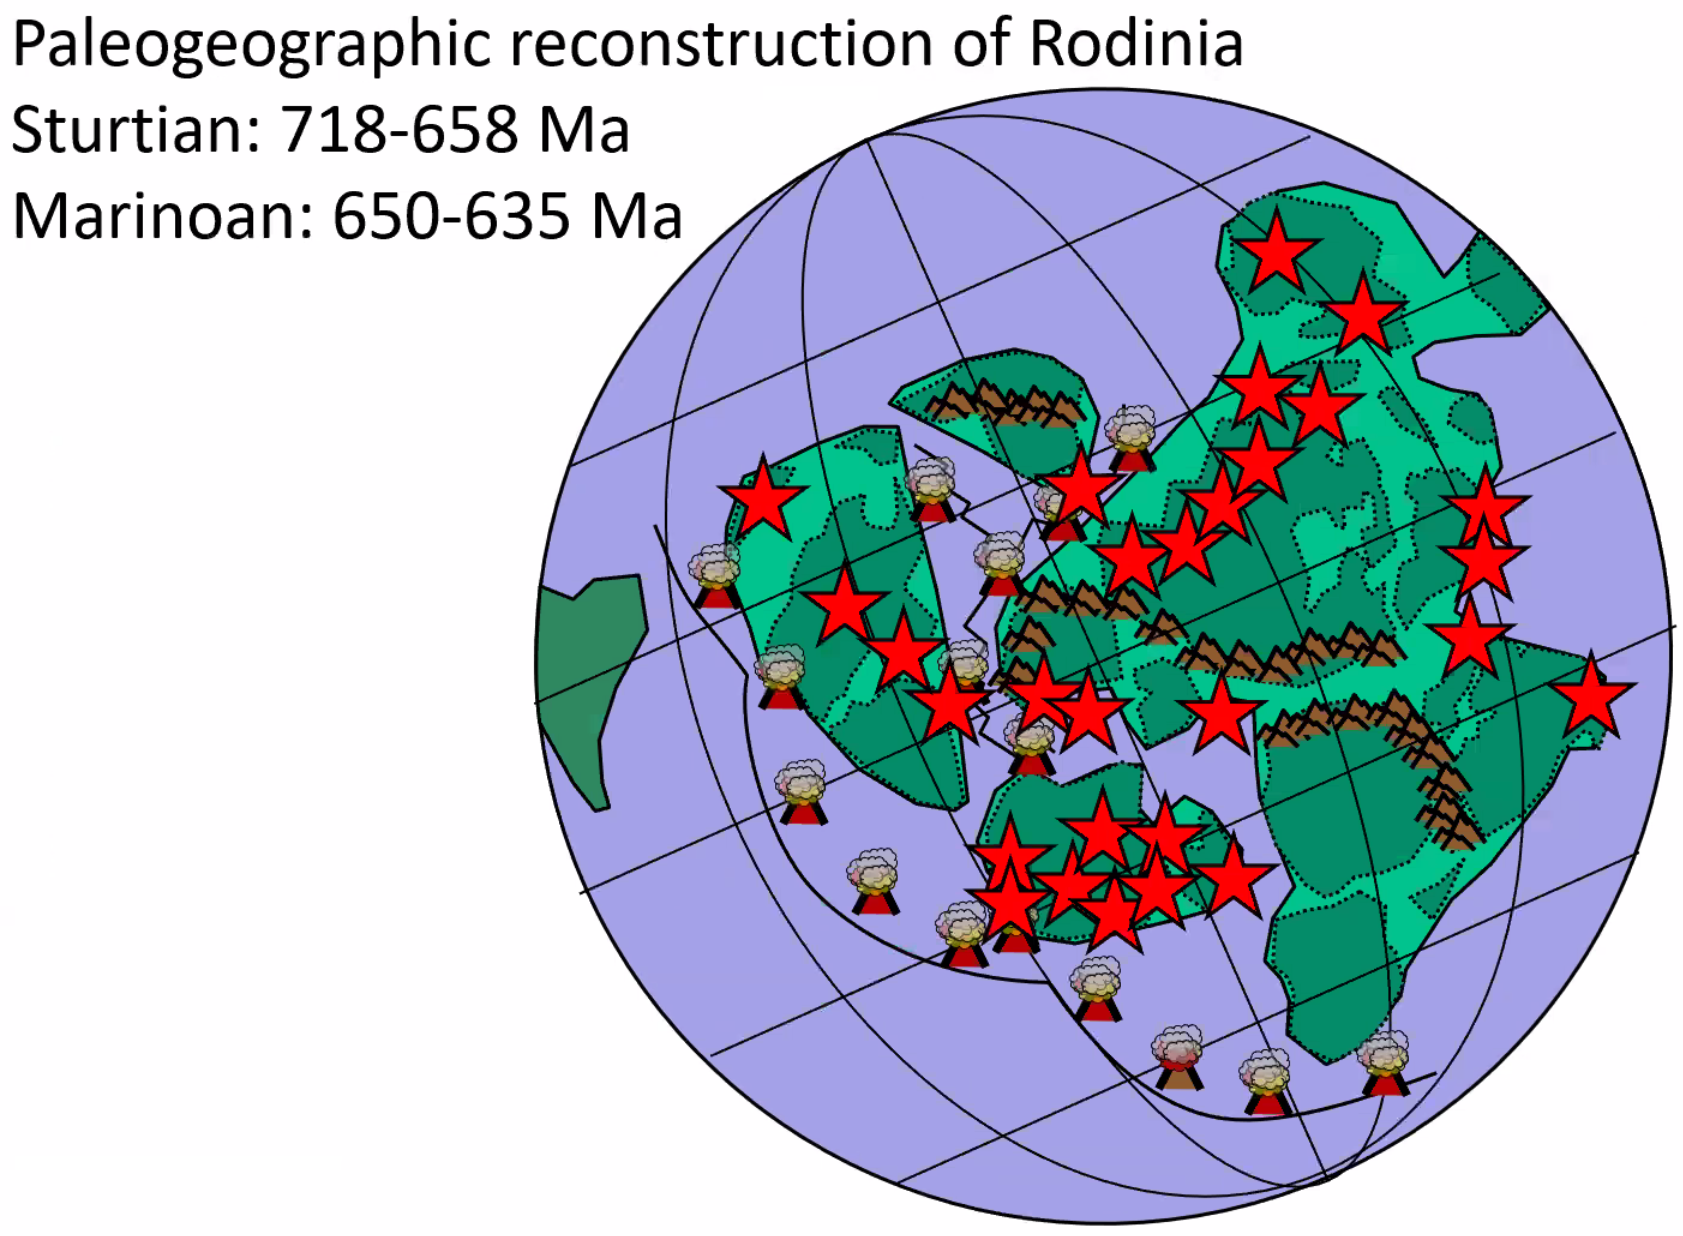
\includegraphics[width=0.75\linewidth]{
    content/img/rodinia_snowball_earth.png}
\end{figure}

So how do we get the glaciers at the equator?

How about \textbf{axial tilt?} It would need to be bigger than $54 \degree$
for the equator to be cooler than the poles. And it wouldn't explain why it
happened twice.

\subsection{Ghaub Formation, Namibia}

\textbf{Till}\footnote{
Till or glacial till is unsorted glacial sediment.

Till is derived from the erosion and entrainment of material by the moving
ice of a glacier. It is deposited some distance down-ice to form terminal,
lateral, medial and ground moraines.

Till is classified into primary deposits, laid down directly by glaciers,
and secondary deposits, reworked by fluvial transport and other processes.
}

\textbf{Cap carbonate}\footnote{
Cap carbonates are layers of distinctively textured carbonate rocks
(either limestone or dolomite) that occur at the uppermost layer of
sedimentary sequences reflecting major glaciations in the geological record.
}

%%%%%%%%%%%%%%%%%%%%%%%%%%%%%%%%%%%%%%%%%%%%%%%%%%%%%%%%%%%%%%%%%%%%%%%%%%%%%%%%
\begin{figure}[H]
    \centering
    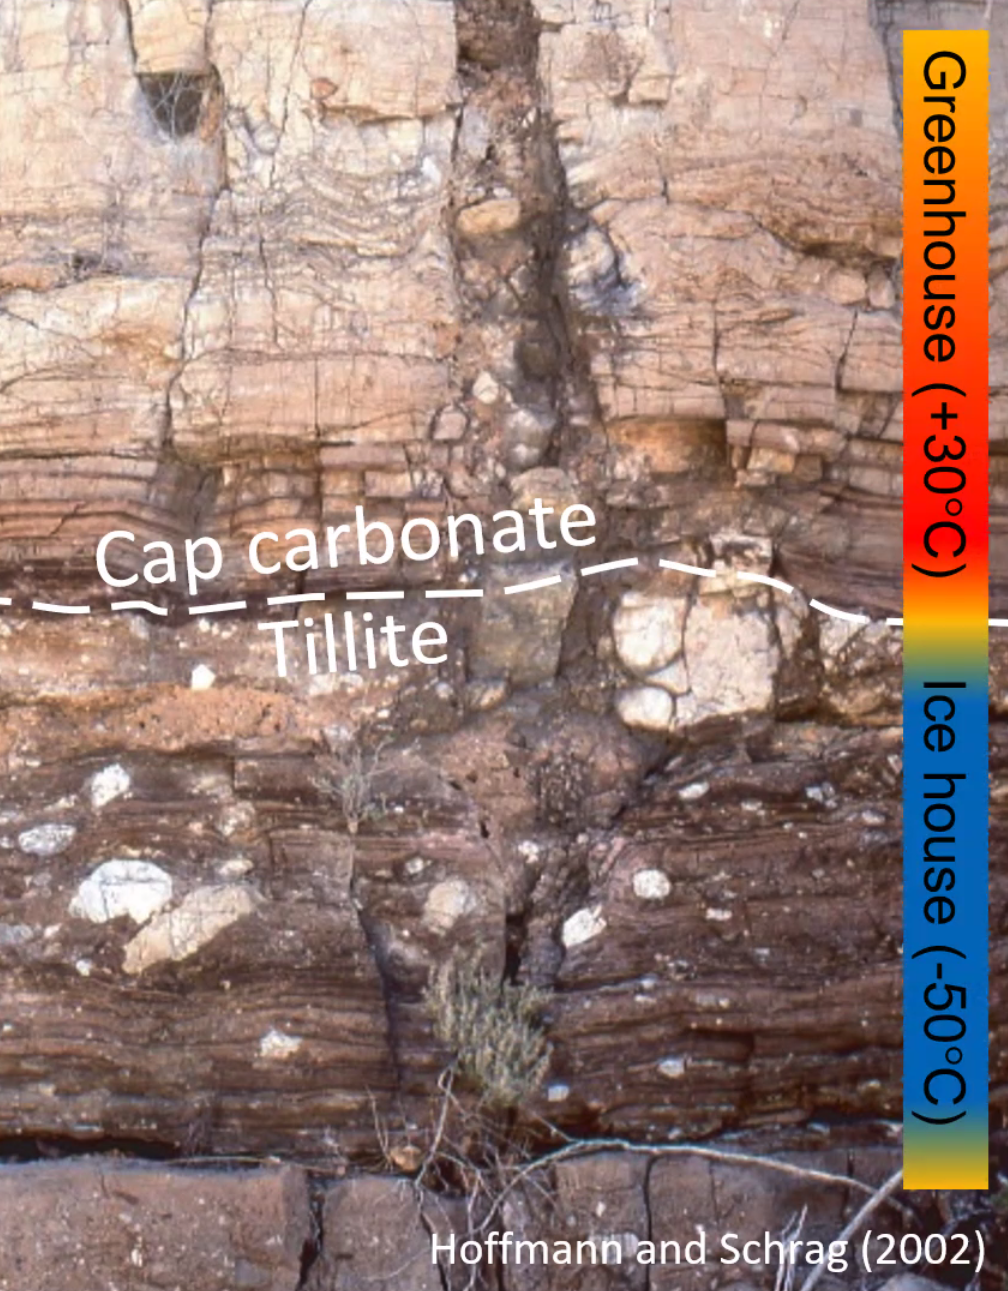
\includegraphics[width=0.75\linewidth]{
    content/img/tillite_and_cap_carbonate.png}
\end{figure}

\subsection{Snowball Earth hypothesis}

Kirschvink (1992) first made the hypothesis but Hoffman popularized it.

Continents in the tropics (with no vegetation because it hadn't evolved yet)
$\rightarrow$
Higher albedo (desert with no vegetation has higher albedo than ocean water)

Mountain building in the tropics $\rightarrow$ Faster weathering

Higher albedo + Faster weathering $\rightarrow$ Earth becomes \textbf{much}
cooler $\rightarrow$ glaciation in the tropics $\rightarrow$ \textbf{even}
higher albedo $\rightarrow$ \textbf{even} faster cooling
$\rightarrow$ Snowball Earth

CO$_2$ from volcanoes $\rightarrow$ increased GH effect

Ash particles from volcanoes $\rightarrow$ Lower albedo

Lower albedo + increased GH effect $\rightarrow$ Earth becomes \textbf{much}
warmer $\rightarrow$ Ice melts $\rightarrow$ \textbf{Even} lower albedo
$\rightarrow$ Ice melts \textbf{faster} $\rightarrow$ Extreme GH

%%%%%%%%%%%%%%%%%%%%%%%%%%%%%%%%%%%%%%%%%%%%%%%%%%%%%%%%%%%%%%%%%%%%%%%%%%%%%%%%

\subsection{Solar radiation}

$T = (E/\delta)^{1/4}$

$E = 342 W.m^{-2}$

$\delta = 5.670367 \times 10^{-8} W.m^{-2}.K^{-4}$

$T = 6\degree$C

Earth's albedo is $\alpha = 30$\% which equals $103W.m^{-2}$

Then the energy left gives $-18\degree$C. GHG contribute $+32\degree$C

\subsection{Solar radiation (716 Myr ago = Onset of Snowball Earth)}

Albedo between 50-95\%. Volcanic ash on ice sheets decreases the albedo.

$E = 160 W.m^{-2}$

$T = -43 \degree$

\subsection{Greenhouse effect (658 Myr = End of Snowball Earth)}

We're looking for how much CO$_2$ would be needed in the atmosphere to exit
the Snowball Earth. Currently (pre-industrial) at 280 ppm the GHG contribute
$32 \degree$ to global temperature.

$\Delta T = 4.3 \ln (C/C_0)$

For 1000 ppm: $\Delta T = 4.3 \ln (1000/280) = 5.5 \degree$

For 10000 ppm: $\Delta T = 4.3 \ln (10000/280) = 15.4 \degree$

For 100000 ppm: $\Delta T = 4.3 \ln (100000/280) = 25.27 \degree$

$T = -11 \degree + 25.c \degree = 14.3 \degree$ at 100000 ppm (10\%
CO$_2$ in the atmosphere)

\subsection{Cap carbonate}

Ca + Mg + CO$_2$ $\rightarrow$ CaMg(CO$_3$)$_2$

\subsection{Iron formations}

Fe + O$_2$ $\rightarrow$ Fe$_2$O$_3$
